%! Author = ${BAIBIZHE}
%! Date = 2020/6/2

% Preamble
\documentclass[18pt]{article}
\author{baibizhe}
\usepackage{indentfirst} 
% Packages
\usepackage{amsmath,geometry}
\usepackage{graphicx}
\geometry{a4paper,scale = 0.8}
\title{CSC338. Homework 3}
% Document
\begin{document}
\maketitle
\vspace{1.5cm}
\noindent
Question 1\\
    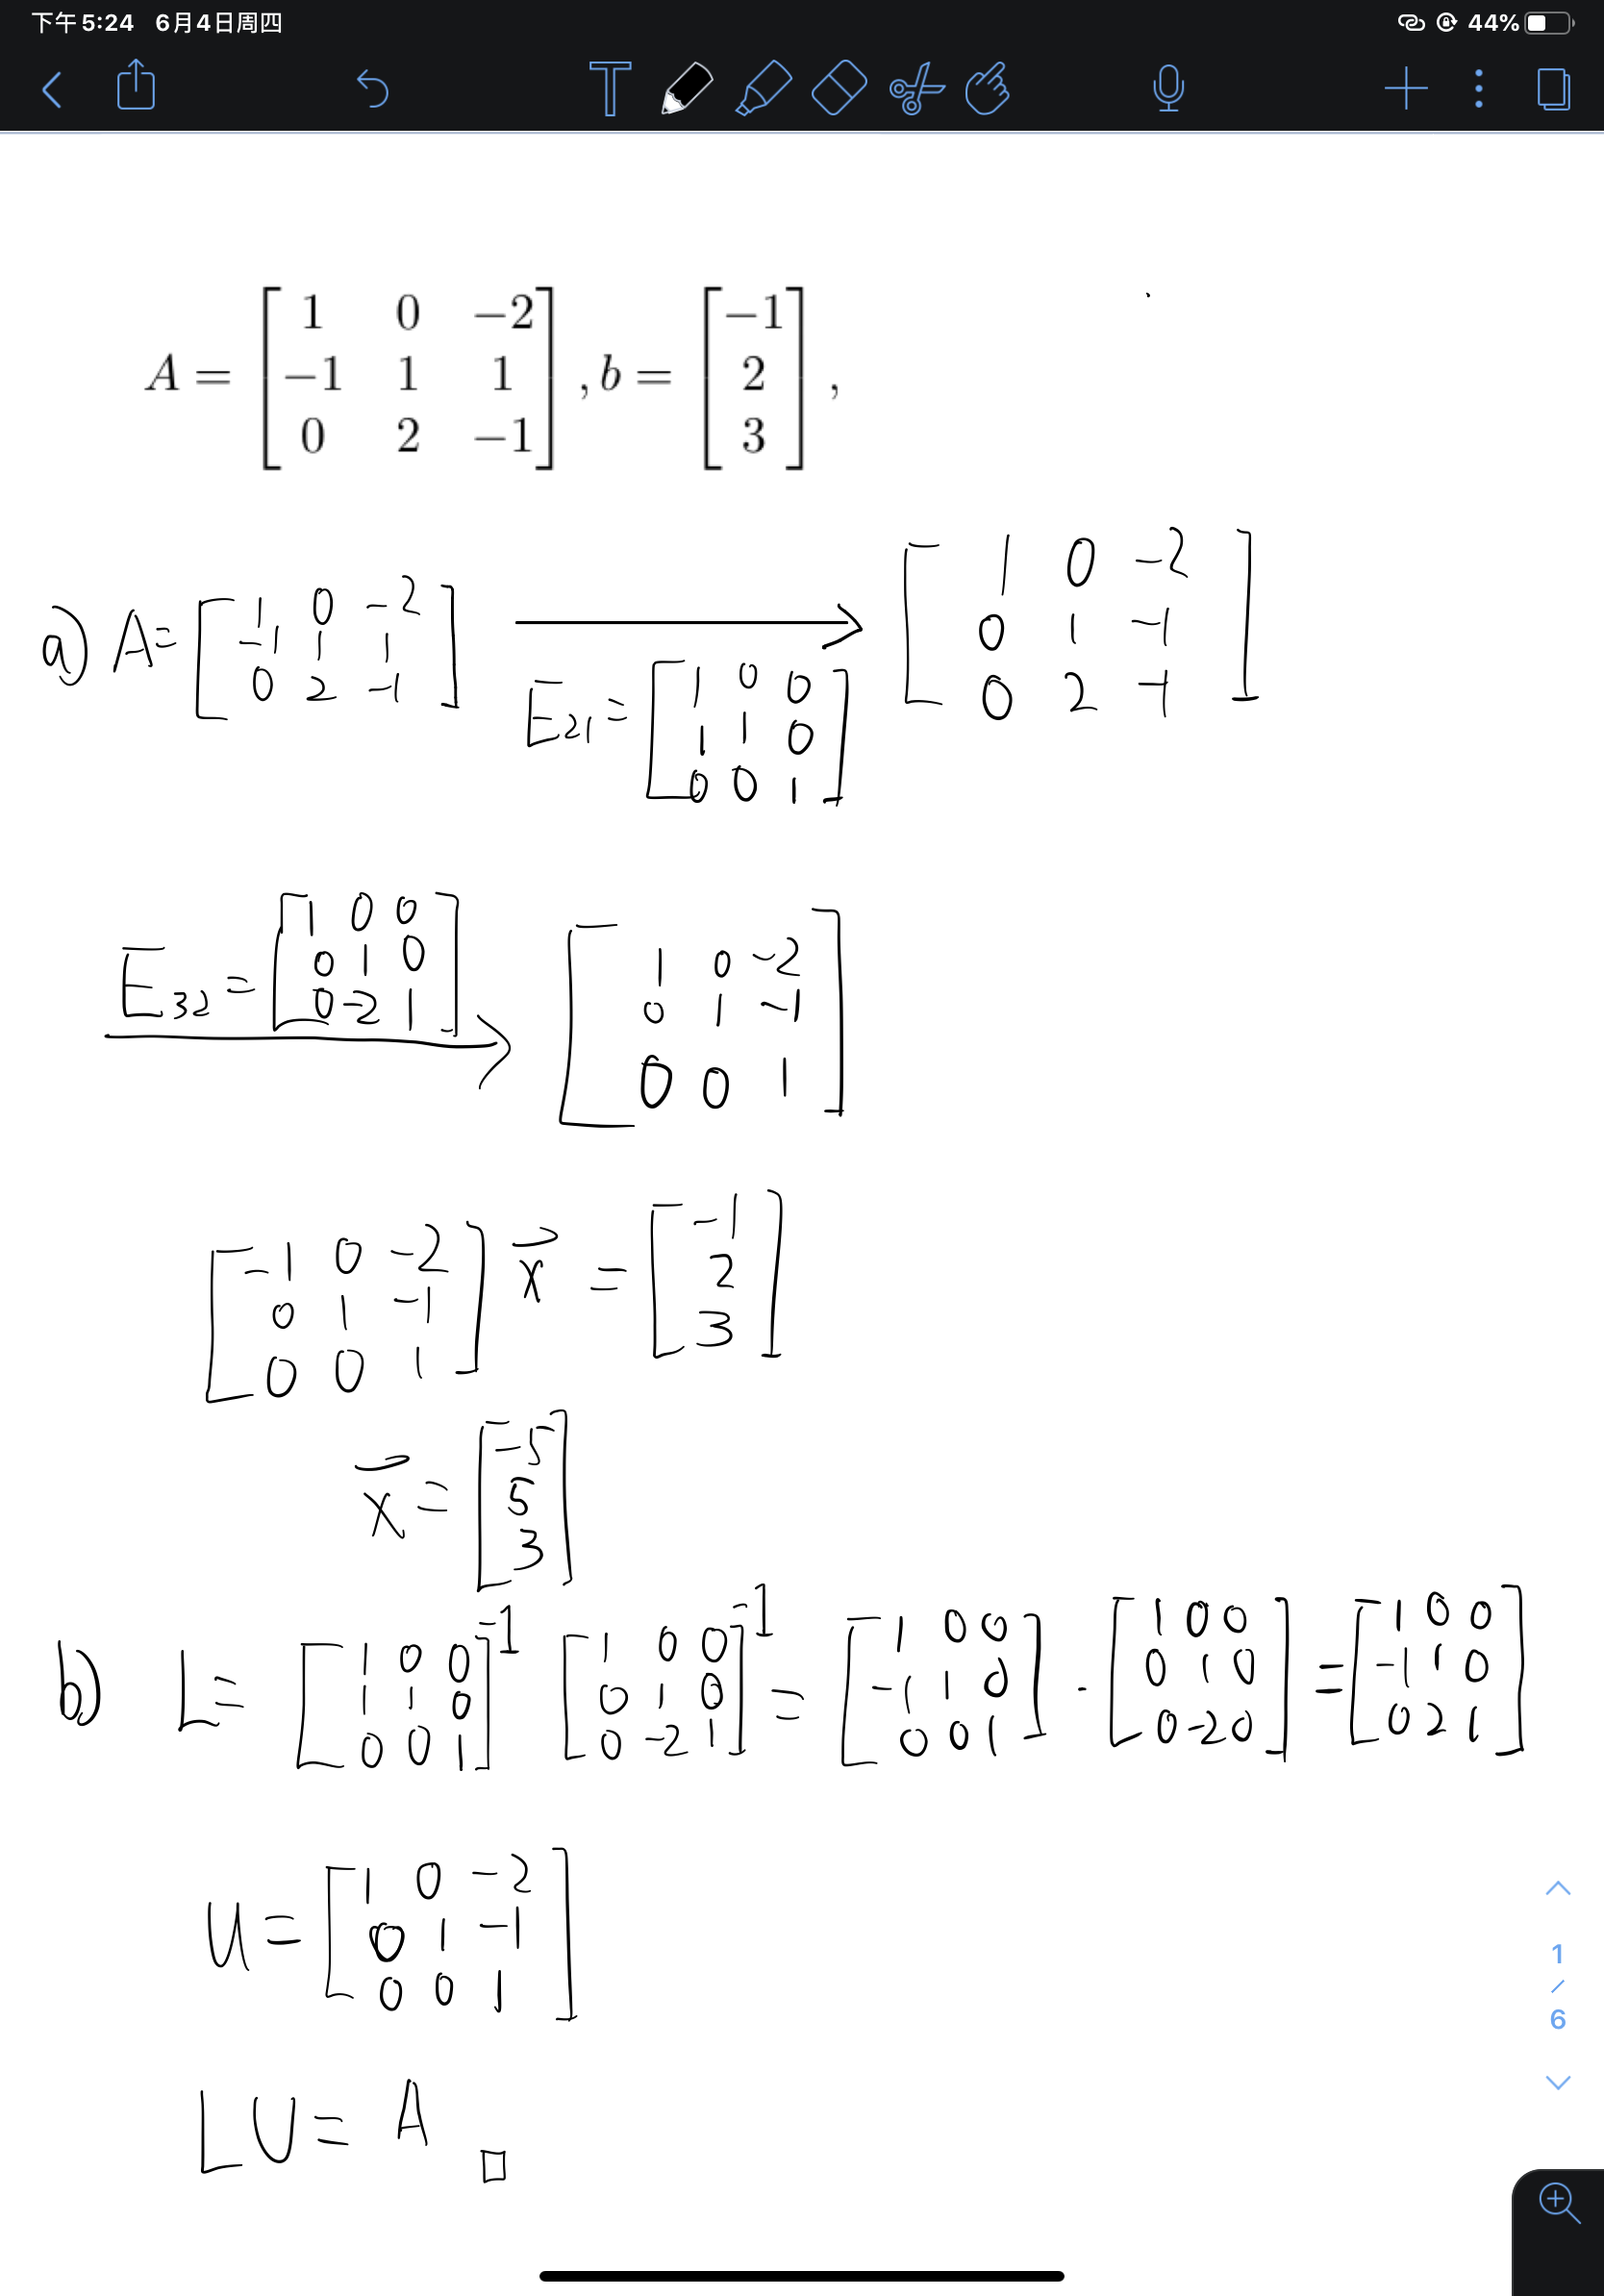
\includegraphics[scale=0.2]{1.PNG}\\
    Question 3\\
For this part prove , i use lemma state in website:\\ https://www.statlect.com/matrix-algebra/matrix-inversion-lemmas\\
$\left(A+u v^{\top}\right)^{-1}=A^{-1}-\frac{1}{1+v^{\top} A^{-1} u} A^{-1} u v^{\top} A^{-1}$\\
    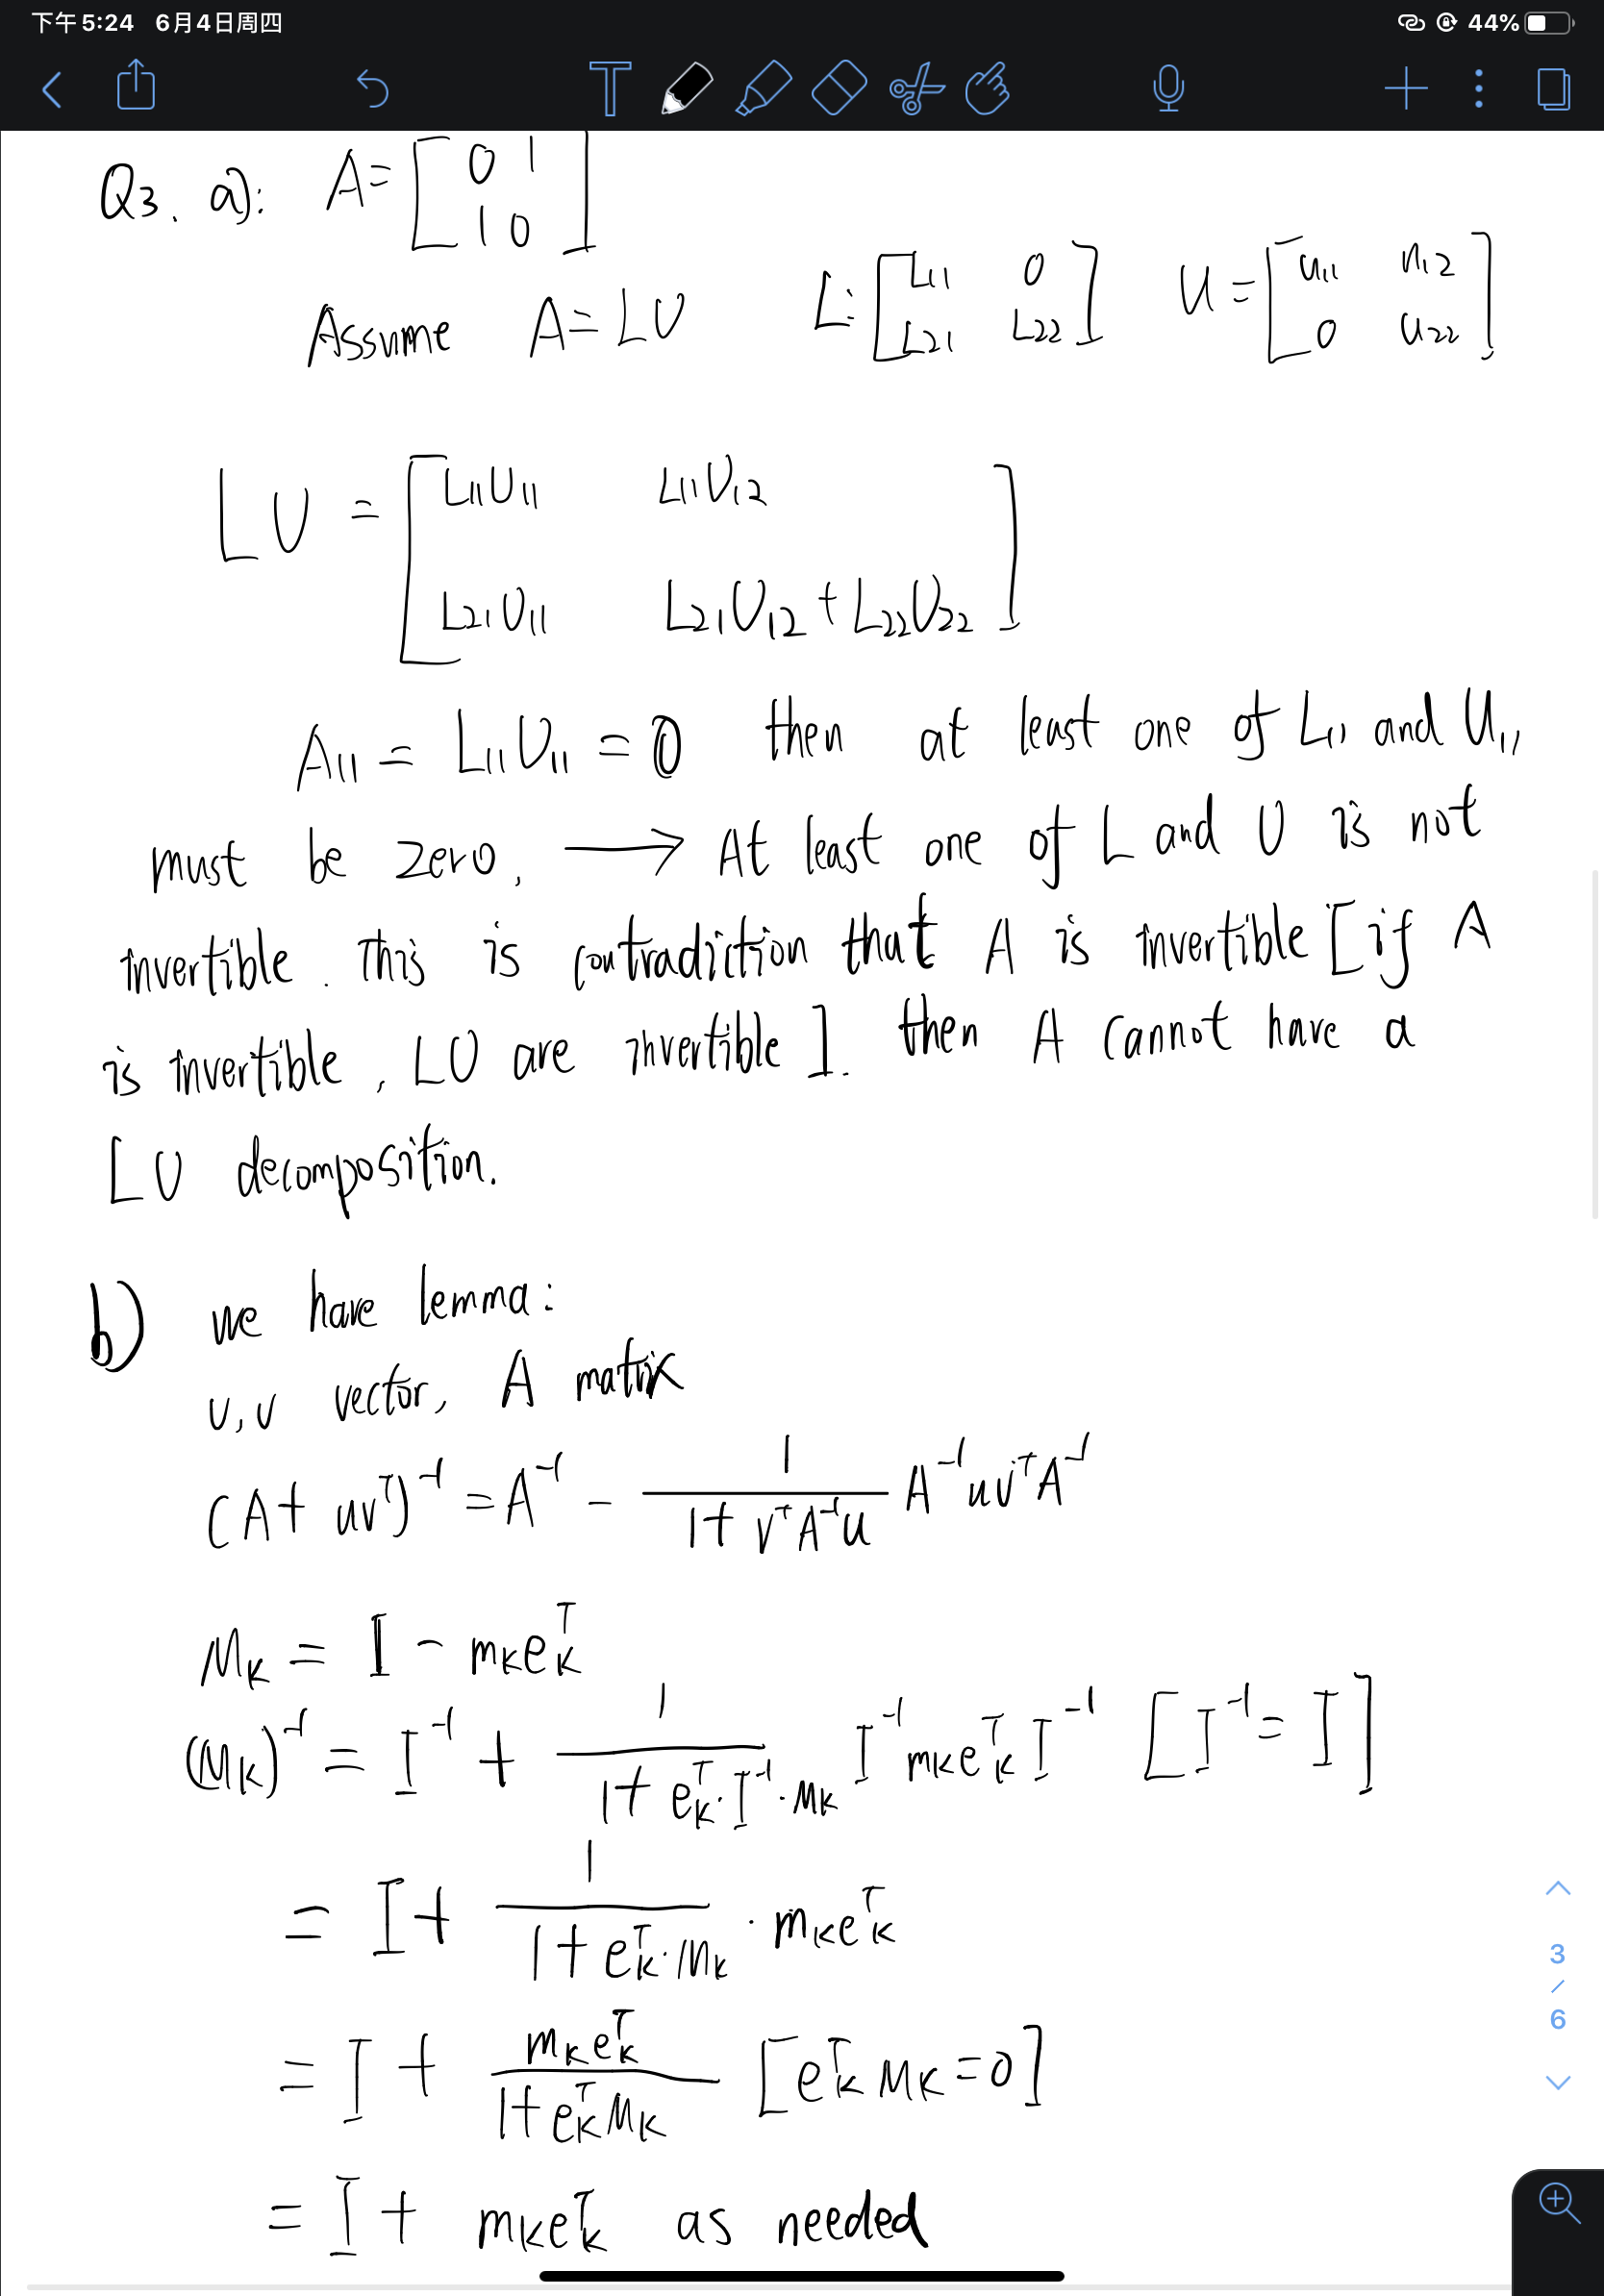
\includegraphics[scale=0.25]{IMG_0831.PNG}\\

\end{document}



